\subtop{Rooted Tree Darstellung}
\begin{description}
	\item[Repräsentant:] Wurzel des zugehörigen Baumes
	\item[\union$(a,b)$:] Anhängen der Wurzel von $a$ an Wurzel von $b$
	\item[\find$(a)$:] Aufsteigen im Baum bis zur Wurzel von $a$
\end{description}
\example{\union(1,2)}{\ \\\up\union$\left(
				\begin{minipage}{2.5cm}
				\usetikzlibrary{positioning}
\begin{tikzpicture}[]
\foreach \x/\y/\z in {1/0/0,5/-1/-1,3/1/-1,7/-1/-2}{
	\node (\x) at (\y,\z) {\x};
}
\foreach \x/\y in {7/5,5/1,3/1}{
	\draw[->](\x)--(\y);
}
\draw[->,loop above](1)to(1);
\end{tikzpicture}
				\end{minipage},
				\begin{minipage}{.5cm}
				\usetikzlibrary{positioning}
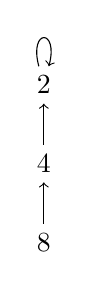
\begin{tikzpicture}[]
\foreach \x/\y/\z in {2/0/0,4/0/-1,8/0/-2}{
	\node (\x) at (\y,\z) {\x};
}
\foreach \x/\y in {4/2,8/4}{
	\draw[->](\x)--(\y);
}
\draw[->,loop above](2)to(2);
\end{tikzpicture}
				\end{minipage}
			\right) = \begin{minipage}{2.5cm}
					\usetikzlibrary{positioning}
\begin{tikzpicture}[]
\foreach \x/\y/\z in {1/0/0,5/-1/-1,3/0/-1,7/-1/-2,2/1/-1,4/1/-2,8/1/-3}{
	\node (\x) at (\y,\z) {\x};
}
\foreach \x/\y in {7/5,5/1,3/1,4/2,8/4,2/1}{
	\draw[->](\x)--(\y);
}
\draw[->,loop above](1)to(1);
\end{tikzpicture}
					\end{minipage}$}
Laufzeiten:
\begin{description}
\item[\makeset:] $\Theta(1)$
\item[\union:] $\Theta(1)$
\item[\find:] Die Laufzeit von \find~ist anhängig von der Höhe des Baumes. Wenn \union~einfach ohne Überprüfung der Höhe der Bäume durchgeführt wird, liegt \find~in $\Theta(n)$.
\end{description}

\subsection{gewichtete Vereinigung (weighted \union)}
Es wird der kleinere Baum an den größeren angehängt. Damit das möglich ist, wird die Größe jedes Baumes folgendermaßen gespeichert: $parent[root] = -size$.\\
Wenn ein Baum aus mehreren \emph{weighted \union} Operationen entstanden ist, so gilt: $h(T) \leq \log |T|$, wobei $h(T)$ die Höhe des Baumes und $|T|$ die Anzahl der Elemente in $T$ ist.

\topbreak

\up Baum $T_j$ wurde an Baum $T_i$ angehängt. Dann gilt: $h(T) = \max(h(T_j)+1,h(T_i))$. Somit entstehen zwei Fälle:
\begin{enumerate}
	\item $h(T_i) > h(T_j)+1 \Rightarrow h(T) =h(T_i) \leq \log |T_i| < T\hspace*{0.5cm} \correct$
	\item $h(T_i) \leq h(T_j)+1\\
	\Rightarrow h(T) = h(T_j)+1 \leq \log |T_j| +1 = \log(2\cdot |T_j|) \leq \log(|T_j|+|T_i|) = \log |T| \hspace*{0.5cm} \correct$
\end{enumerate}
$\Rightarrow $ Eine Sequenz von $n$ \makeset-Operationen und $m$ \emph{weighted} \union- und \find-Operationen, kann in $\BigO(m \log n)$ ausgeführt werden.

\subsection{\find~mit "Path Compression"}
Bei der Suche nach dem Schlüssel $k$ ändern wir für alle Knoten auf dem Pfad von $root$ zu $a$ den Zeiger zum Vorgänger ($parent[x] \leftarrow root$, $x$ liegt auf dem Pfad von $root$ zu $a$).
\example{\find(9)}{\ \\
	\begin{tabular}{ll}
	Vor der Suche nach 9: & Nach der Suche nach 9: \\
	\usetikzlibrary{positioning}
\begin{tikzpicture}[]
\foreach \x/\y/\z in {-9/0/1,1/0/0,2/-1/-1,3/0/-1,5/0/-2,4/1.5/-1,6/1/-2,7/2/-2,8/1.5/-3,9/2.5/-3}{
	\node (\x) at (\y,\z) {\x};
}
\foreach \x/\y in {1/-9,2/1,3/1,4/1,5/3,6/4,7/4,8/7,9/7}{
	\draw[->](\x)--(\y);
}
\end{tikzpicture} & \usetikzlibrary{positioning}
\begin{tikzpicture}[]
\foreach \x/\y/\z in {-9/0/1,1/0/0,2/-2/-1,3/-1/-1,5/-1/-2,4/0/-1,6/0/-2,7/1/-1,8/1/-2,9/2/-1}{
	\node (\x) at (\y,\z) {\x};
}
\foreach \x/\y in {1/-9,2/1,3/1,4/1,5/3,6/4,7/1,8/7,9/1}{
	\draw[->](\x)--(\y);
}
\node(phan) at(0,-3){\phantom{phan}};
\end{tikzpicture} \\
	\end{tabular}
}
Laufzeiten:
\begin{description}
	\item[\find:] $\Theta(\log n)$
	\item[\union:] $\Theta(1)$
	\item[\makeset:] $\Theta(1)$
\end{description}
Mit der Anwendung der amortisierten Kosten erhält man jedoch folgendes:
\begin{description}
	\item[\find:] $\Theta(\log^{*} n)$
\end{description}
Wobei folgendes gilt (\textbf{iterativer Logarithmus}):
\[\log^{*} n = \min \{j \geq 0;\log^{(j)} n \leq 1\}\]
sowie
\[\log^{(i)} n = \left\{ \begin{array}{ll}
		n & \text{falls } i=0\\
		\log(\log^{(i-1)}n) & \text{falls } i>0 \text{ und } \log^{(i-1)} >0 \text{ definiert}\\
		\text{undefiniert}&\text{sonst}
	\end{array}\right. \]
Der \textbf{rank} $r(v)$ eines Knotes $v$ entspricht der Höhe seines Teilbaumes, gewurzelt bei $v$. Somit gilt
\[r(v) \leq \log n,~\forall v \in V\]
Eine \textbf{Rank}-Gruppe $R_j$ ist eine Menge von Knoten für die gilt:
\[R_j=\left\{
	\begin{array}{ll}
		\{v | \log^{(j+1)} n > r(v) \leq \log^{(j)}n\} & \text{falls } \log^{(j+1)} n \text{ definiert ist}\\
		\{v | r(v) = 0\} & \text{falls } \log^{(j)} n < 1 \text{ definiert ist}\\
		\emptyset & \text{sonst}
	\end{array}
\right.\]
\topbreak
\up
\example{r(1)=5, r(21)=4, r(11)=r(31)=3\text{, grüne: }r()=2\text{, blaue: }r()=1\text{, rote: }r()=0}{
$\text{Sowie }R_1\text{ sind die schwarzen Knoten,}$\\
$R_2\text{ sind die grünen Knoten,}\\R_3\text{ sind die blauen Knoten,}\\R_4\text{ sind die roten Knoten.}$\ \\
\usetikzlibrary{positioning}
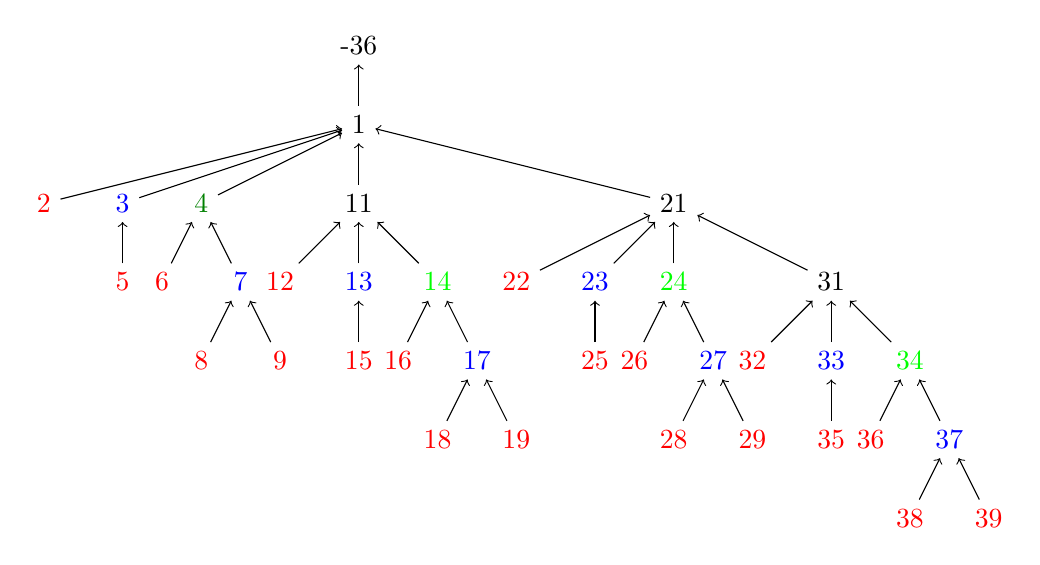
\begin{tikzpicture}[node distance=0.5cm]
\def\col{black}
\foreach \x/\y/\z in {-36/0/1,1/0/0,2/-4/-1,3/-3/-1,4/-2/-1,11/0/-1,21/4/-1,31/6/-2}{
	\ifnum\x=2\edef\col{red}\fi
	\ifnum\x=3\edef\col{blue}\fi
	\ifnum\x=4\edef\col{green!50!black}\fi
	\node[color=\col] (\x) at (\y,\z) {\x};
}

\def\level{2}
\foreach \x/\y in {7/-1.5,13/0,17/1.5,23/3,27/4.5,33/6,37/7.5}{
	\edef\col{blue}
	\ifnum\x=17 \edef\level{3}\fi
	\ifnum\x>23 \edef\level{3}\fi
	\ifnum\x=37 \edef\level{4}\fi
	\node[color=\col](\x)at(\y,-\level){\x};
}
\foreach \x/\y in {14/1,24/4,34/7}{
	\edef\col{green}
	\ifnum\x>24 \edef\level{3}\fi
	\node[color=\col](\x)at(\y,-\level){\x};
}
\foreach[count=\c] \x/\y in {5/-3,6/-2.5,12/-1,22/2,8/-2,9/-1,15/0,16/0.5,25/3,26/3.5,32/5,18/1,19/2,28/4,29/5,35/6,36/6.5,38/7,39/8}{
	\edef\col{red}
	\ifnum\c>4 \edef\level{3}\fi	
	\ifnum\c>11 \edef\level{4}\fi
	\ifnum\c>17 \edef\level{5}\fi
	\node[color=\col](\x)at(\y,-\level){\x};
}
\def\m{}
\foreach[count=\c] \x/\y in {-36,1,1,1,3,4,4,7,7,0,1,11,11,11,13,14,14,17,17,0,1,21,21,21,23,24,24,27,27,0,21,31,31,31,33,34,34,37,37}{
	\pgfmathparse{Mod(\c,10)==0?1:0}
	\ifnum\pgfmathresult>0 
	\else{
		\draw[->](\c)--(\x);
	}
	\fi
}
\end{tikzpicture}
}
Alle ranks steigen zur jeder Zeit der Sequenz auf dem Weg eines Knotens zur Wurzel strikt monoton an (auf einem Pfad vom Knoten zur Wurzel).
\vspace*{-0.5\baselineskip}
\Proof
Zu einem bestimmten Punkt setzen wir für einen Knoten $v$: $parent[v] \leftarrow w$ durch die Pfadkompression (davor war $v$ in einem Teilbaum von $w$). Somit war vorher schon $r(v) < r(w)$.\\\\
Es gibt höchstens $\frac{n}{2^r}$ Knoten vom rank $r$.
\vspace*{-0.5\baselineskip}
\Proof
$T_v$ ist Teilbaum gewurzelt bei $v$ vom rank $r$ im Wald $T'$. Dann gilt
\[r=h(T_v)\leq \log |T_v|~~\Rightarrow |T_v|\geq 2^r\]
Da zwei Teilbäume mit demselben rank disjunkt sind und es insgesamt $n$ Knoten gibt folgt daraus, dass es höchstens $\frac{n}{2^r}$ Knoten pro rank gibt.\\\\
\emph{Beginn der amortisierten Analyse:}
\begin{enumerate}
	\item Originalsequenz ($\sigma$)
	\item Hinzurechnen der Kosten einer Operation \find$(x)$ zu der Operation für das Bewegen der Knoten (eine Einheit für das Durchlaufen der Knoten auf einem Pfad $x$ zur Wurzel (inklusive $x$, ohne Wurzel und Vorgänger der Wurzel) und eine Einheit für das Bewegen der Knoten)
	\item zwei Arten von Bewegungen:
		\begin{description}
			\item[Typ A:] Vor der Bewegung gilt $R_i(v), R_j(parent[v]), i\neq j$
			\item[Typ B:] Vor der Bewegung gilt $R_i(v), R_j(parent[v]), i=j$
		\end{description}
	\item es gibt höchstens $\log^{*} n+1$ nicht-leere Rank-Gruppen
	\item weil der rank eines Knotens auf dem Weg zur Wurzel ansteigt folgt, dass es höchstens $\log^{*}n$ Bewegungen vom \emph{Typ A} gibt
	\item es gibt weniger als $\log^{j}n$ Bewegungen in der Rank-Gruppe $R_j$
	\item es gibt höchstens $\frac{n}{2^r}$ Knoten pro rank
\end{enumerate}
\topbreak
\up\ \\Hieraus folgt:\\
$\begin{array}{lcl}
	|R_j| & < &\sum\limits_{i=\ceil{\log^{(j+1)} n}}^{\infty}\dfrac{n}{2^i}\\
	& = & \dfrac{n}{2^{\ceil{\log^{(j+1)} n}}} \cdot \sum\limits_{i=0}^{\infty}\dfrac{1}{2^i}\\
	& \leq & \dfrac{2n}{2^{\log^{(j+1)} n}}\\
	& = & \dfrac{2n}{2^{\log(\log^{(j)} n)}}\\
	& = & \dfrac{2n}{\log^{(j)} n}
\end{array}$\\
Somit gibt es $|R_j| \cdot \log^{(j)} = 2n$ Bewegungen vom Typ B pro Rank-Gruppe.\\
$\Rightarrow 2n\cdot \log^{*}n+1$ Bewegungen vom Typ B.\\
\emph{Zusammenfassend:}\\
Eine Sequenz von $m$ Operationen \makeset, gewichtete \union~und \find~mit Pfadkompression ($n$ sind \makeset-Operationen) kann in $\BigO(m\log^{*}n)$ ausgeführt werden.
\subsection{inverse Ackermannfunktion}
Wächst langsamer als der iterative Logarithmus, die $m$ Operationen können in $\BigO(m\alpha(m,n))$ ausgeführt werden, wobei $\alpha$ eine Variante der inversen Ackermannfunktion ist.\\\\